\usetikzlibrary{calc}
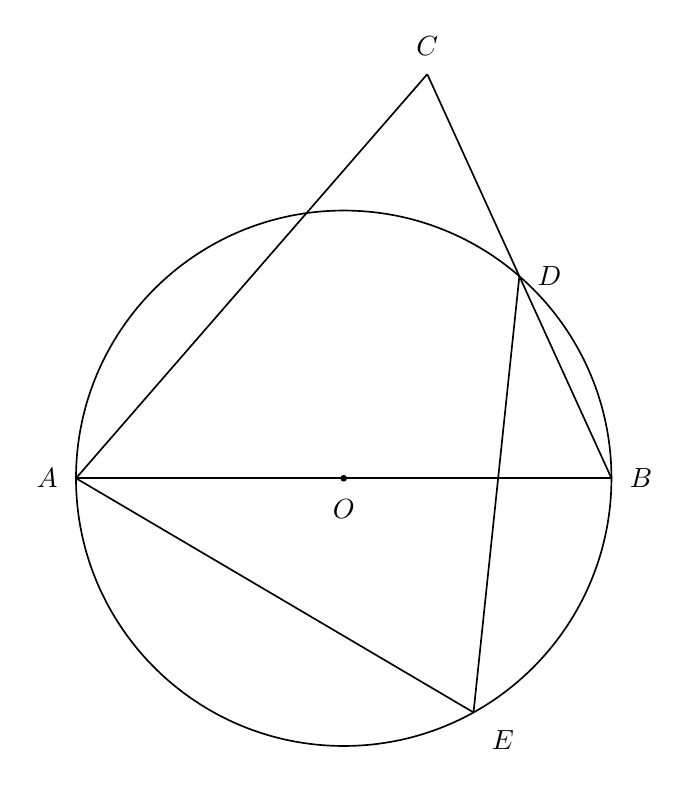
\begin{tikzpicture}[x=1cm,y=1cm,line width=.6pt,font=\normalsize]
\coordinate (O) at (0,0);
\coordinate (A) at (-3.4,0);
\coordinate (B) at (3.4,0);
\coordinate (D) at (2.230601,2.566014);
\coordinate (E) at (1.648354,-2.973708);
\coordinate (C) at (1.061202,5.132028);
\draw (O) circle[radius=3.4cm];
\draw (A)--(B);
\draw (B)--(C);
\draw (A)--(C);
\draw (D)--(E);
\draw (A)--(E);
\fill (O) circle[radius=1.2pt];
\node[left=3pt] at (A) {$A$};
\node[right=3pt] at (B) {$B$};
\node[above=3pt] at (C) {$C$};
\node[right=3pt] at (D) {$D$};
\node[below right=3pt] at (E) {$E$};
\node[below=4pt] at (O) {$O$};
\end{tikzpicture}
